\documentclass[12pt,a4paper]{article}
\usepackage{CJK}
\usepackage{amsmath,epsfig,algorithm,algorithmic}
\setlength\parindent{0pt} % Removes all indentation from paragraphs - comment this line for an assignment with lots of text

\begin{document}

\begin{CJK*}{UTF8}{kai}

\title{
\huge Assignment 1 \\ % The assignment title
}
\author{Luo Zhiyi (0130339024)}
\date{Spring 2014}
\maketitle

%符号说明:
%
%对于单个神经元来说,有:
%$ a_{j}^{(k)} = f((\sum_{i=1}^{N_{k-1}}(u_{ji}^{(k)})+v_{ji}^{k}a_i^{(k-1)}+b_j^{(k)}))$
%
%
%现考虑神经元
%%{\setlength\arraycolsep{2pt}
%%\begin{eqnarray}
%
%%\begin{equation}\label{(1-1)}
%%\begin{split}
%%%$
%%\frac{\partial{z_j^{(l+1)}}}{\partial{z_i^{(l)}}} & =
%%\frac{\partial{(\sum_{m=1}^{N^(l)}u_{jm}^{(l+1)}(a_{m}^{(l)})^2+v_{jm}^{(l+1)}a_m^{(l)}+b_j^{(l+1)})}}
%%{\partial{z_i^{(l)}}}\\
%%& = 2a_i^{(l)}u_{ji}^{(l+1)}\frac{\partial{a_i^{(l)}}}{\partial{z_i^{(l)}}}+
%%v_{ji}^{(l+1)}\frac{\partial{a_i^{(l)}}}{\partial{z_i^{(l)}}}\\
%%& = (2u_{ji}^{(l+1)}a_i^{(l)}+v_{ji}^{(l+1)})\frac{\partial{a_i^{(l)}}}{\partial{z_i^{(l)}}}
%%%$
%%\end{split}
%%\end{equation}
%
%用向量形式表示得到:
%
%\begin{equation}\label{(1-2)}
%\frac{\partial{\mathbf{z}^{(l+1)}}}{\partial{\mathbf{z}^{(l)}}}=
%2\mathbf{u}^{(l+1)}\mathbf{a}^{(l)}+\mathbf{v}^{(l+1)}\mathbf{F}^{(l)}(\mathbf{z}^{(l)})
%\end{equation}
%其中,
%
%\begin{equation}\label{(1-3)}
%\begin{split}
%      \mathbf{F}^{(l)} & =  \mathbf{diag}({f^{'}(z_{i}^{(l)})}), \quad i=1,2,...,N_l\\
%      \mathbf{G}^{(l)} & =  \mathbf{diag}(z_i^{(l)}f^{'}(z_i^{(l)})), \quad i=1,2,...,N_l
%\end{split}
%\end{equation}
%
%sigmoid函数的导数为 $f^{'}(z)=f(z)(1-f(z))$
%
%\begin{equation}\label{(1-4)}
%\frac{\partial{\mathbf{J}}}{\partial{\mathbf{z}^{(l)}}}=
%(\frac{\partial{\mathbf{z}^{(l+1)}}}{\partial{\mathbf{z}^{(l)}}})^{T}
%\frac{\partial{\mathbf{J}}}{\partial{\mathbf{z^{(l+1)}}}}
%\end{equation}
%
%设$\delta^{(l)}=\frac{\partial{\mathbf{J}}}{\partial{\mathbf{z}^{(l)}}}$,则有
%\begin{equation}\label{(1-5)}
%\delta^{(l+1)} = \delta^{(l)}(\frac{\partial{\mathbf{z}^{(l+1)}}}{\partial{\mathbf{z}^{(l)}}})^{T}
%\end{equation}
%对于在线学习(on-line learning),对于第$m$个样本,进行一次参数更新。这里我们将$J(U,V,b)$简写为$J$。因为神经网络共有$M$层,所以先要求出$\delta^{(M)}$, 对于输出层$M$ 层的第i个单元的cost function 有:$J_i = (y_i-a_i^{(M)})^2$, 则
%
%\begin{equation}
%\begin{split}
%    \delta_i^{(M)} = -2(y_i - a_i^{(M)})f^{(M)}(z_i^{(M)})
%\end{split}
%\end{equation}
%
%\begin{equation}
%\begin{split}
%    \mathbf{\delta}_i^{(M)} = -2\mathbf{F}^{(M)}(\mathbf{z}^{(M)})(\mathbf{y} - \mathbf{a}^{(M)})
%\end{split}
%\end{equation}
%
%每来一个样本都对参数$\mathbf{u}$,$\mathbf{v}$,$\mathbf{b}$进行更新。
%
%\begin{equation}
%\begin{split}
%\mathbf{U}^{(l)} &:= \mathbf{U^{(l)}} - 2\alpha \delta^{(l+1)}(a^{(l)})^{T}\mathbf{diag}(a_i^{(l)}) \\
%\mathbf{V}^{(l)} &:= \mathbf{V^{(l)}} - \delta^{(l)} (a^{(l)})^{T}
%\end{split}
%\end{equation}
%
%$\alpha$ 为learning rate
%批处理学习(batch learning)
%
%\begin{equation}
%\theta = ln(\frac{u}{1-u})
%\end{equation}
\end{CJK*}

\section{Introduction}
This is the report of assignment1 for neural network design course.
The problem is to solve the two-spiral classification problem by implementing a multi-layer quadratic perception(MLQP) network with one hidden layer. I implement both online learning and batch learning ways to train the MLQPs model with the training data.
This report consists of derivation of the back-propagation algorithms for MLQPs, description of the implementation and the analysis of experiment result applying the model on the two-spiral problem.

%\begin{figure}
%\centering
%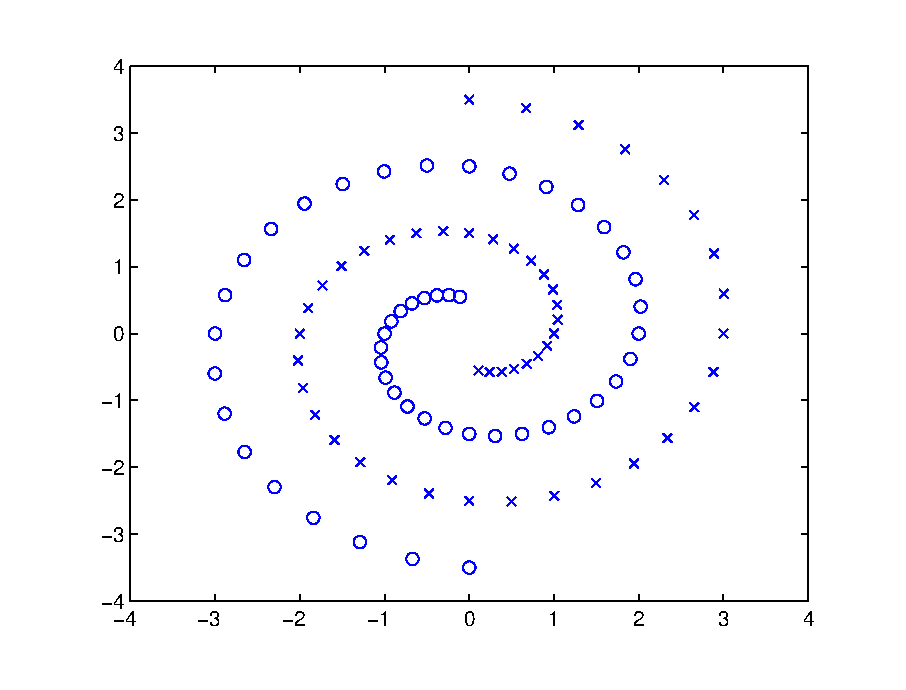
\epsfig{file=trainExamples.eps,width=0.9\columnwidth}
%\caption{Training set examples plotting}
%\end{figure}


\section{Multi-layer Quadratic Perceptron}
\subsection{MLQPs Formulation}
In this report, I use $u_{i,j}^{(l)}$ and $v_{i,j}^{(l)}$ to denote
the weights connecting the $i$th unit in the layer $l$ to the $j$th unit in the layer $l+1$, $b_{i}^{(l)}$ is the basis of the $i$th unit in the layer $l$. $N^{(l)}$ is the number of units in $l$th layer ($1<=l<=M$), and f(.) is the sigmoid activate function:$f(z)= \frac{1}{1+e^{-z}}$ and $f^{'}(z) = f(z)(1-f(z))$.

In fact, our MLQPs is an example of \textbf{feedforward} neural network. I'll introduce the notations and formulations in MLQPs through feedforward calculation. Figure 2 describes a brief structure of the implemented MLQPs. For the feedforward process, the computation that the MLQPs represents is given by:
\begin{equation}\label{unit}
\begin{split}
z_{j}^{(l)} &= \sum_{i=1}^{N^{(l-1)}}(u_{ji}^{(l)})(a_i^{(l-1)})^2+v_{ji}^{l}a_i^{(l-1)}+b_j^{(l)}
\\
a_{j}^{(l)} &= f(z_{j}^{(l)})
\end{split}
\end{equation}

\subsection{Cost Function}
Suppose we have a given training set, say {$(\mathbf{x}^{(1)},y^{(1)}),(\mathbf{x}^{(2)},y{(2)}),...,(\mathbf{x}^{(m)},y{(m)})$}.
In detail, the $\mathbf{x}^{(i)}$ denotes the $i$th example's feature vector, contains the x-coordinate and y-coordinate information.
Since the two-spiral classification is a binary classification problem, it implies that the data follows Bernoulli distribution, so I use the following function form to be the cost function for a single example$(\mathbf{x}^{(i)},y^{(i)})$:
\begin{equation}
J(U,V,b;\mathbf{x}^{(i)},y^{(i)}) = -(y^{(i)}log(h_\theta(\mathbf{x}^{(i)}))
+ (1-y^{(i)})log(1-h_\theta(\mathbf{x}^{(i)}))
\end{equation}
where the $h_\theta(\mathbf{x}^{(i)})$ denotes the MLQPs' output for example $(\mathbf{x}^{(i)},y^{(i)})$. In binary classification problem, a simple interpretation of  $h_\theta(\mathbf{x}^{(i)})$ is the probability of $y^{(i)}$ equals to 1, given the parameter $\theta$ and data $\mathbf{x}^{(i)}$. I also add the regularization term to avoid over-fitting problem. I set the weight decay parameter $\lambda$ to be 0.0001 by experience. Given a training set of $m$ examples, I then define the overall cost function to be

\begin{equation}
J(U,V,b) = [-\frac{1}{m}\sum_{i=1}^{m}{J(U,V,b)}] + \frac{\lambda}{2}\parallel{U}\parallel_{2}^{2} +\frac{\lambda}{2}\parallel{V}\parallel_{2}^{2}
\end{equation}
Our goal is to minimize the $J(U,V,b)$ as a function of $U$, $V$ and $b$. To train the MLQPs model, I will initialize each parameter to a small random value close to zero, and then apply an optimization algorithm such as batch gradient descent and online gradient descent.

\subsection{Back-propagation algorithm}
We will now describe the back propagation algorithm, which gives an efficient way to compute the partial derivatives when updating the model parameters.

Intuitively, we have the following formulation of the partial derivatives calculation:

\begin{equation}
\begin{split}
\frac{\partial{J}}{\partial{U}} &= \frac{\partial{J}}{\partial{z^{(l+1)}}}
\frac{\partial{z^{(l+1)}}}{\partial{z^{(l)}}}\frac{\partial{z^{(l)}}}{\partial{U}}
\\
\frac{\partial{J}}{\partial{V}} &= \frac{\partial{J}}{\partial{z^{(l+1)}}}
\frac{\partial{z^{(l+1)}}}{\partial{z^{(l)}}}\frac{\partial{z^{(l)}}}{\partial{V}}
\\
\frac{\partial{J}}{\partial{b}} &= \frac{\partial{J}}{\partial{z^{(l+1)}}}
\frac{\partial{z^{(l+1)}}}{\partial{z^{(l)}}}\frac{\partial{z^{(l)}}}{\partial{b}}
\end{split}
\end{equation}

More formally, we do the following derivation for each unit(Here we only consider the parameter $U$, $V$ and $b$ are similar):

\begin{equation}
\frac{\partial{J}}{\partial{u_{ij}^{(l)}}}=
\frac{\partial{J}}{\partial{z_j^{(l+1)}}}
\frac{\partial{z_j^{(l+1)}}}{\partial{u_{ij}^{(l)}}}
\end{equation}

\begin{equation}
\frac{\partial{J}}{\partial{z_j^{(l)}}}=
\frac{\partial{J}}{\partial{z_i^{(l+1)}}}
\frac{\partial{z_i^{(l+1)}}}{\partial{a_j^{(l)}}}
\frac{\partial{a_j^{(l)}}}{\partial{z_j^{(l)}}}
\end{equation}
We can obtain the following formulation through \label{unit}:
\begin{equation}
\frac{\partial{z_i^{(l+1)}}}{\partial{a_j^{(l)}}}=
2u_{ji^{(l)}}a_j^{(l)}+v_{ji}^{(l)} + v_{ji}^{(l)}a_j^{(l)}
\end{equation}

\begin{equation}
\frac{\partial{a_j^{(i)}}}{\partial{z_j^{(l)}}}=
f(z_j^{(l)})(1-f(z_j^{(l)}))
\end{equation}
Let us use $\delta_j^{(l)}$ short for $\frac{\partial{J}}{\partial{z_j^{(l)}}}$.
Then, we will get:

\begin{equation}
\delta_j^{(l)} = \delta_i^{(l+1)}
(2u_{ji^{(l)}}a_j^{(l)}+v_{ji}^{(l)} + v_{ji}^{(l)}a_j^{(l)})
f(z_j^{(l)})(1-f(z_j^{(l)}))
\end{equation}
So,
\begin{equation}
\frac{\partial{J}}{\partial{u_{ij}^{(l)}}}=
\delta_i^{(l+1)}lalalalallalalllalallalalal
\end{equation}

Now, we know how to calculate the gradient of model parameters $U$, $V$ and $b$.

In detail, the derivation about partial derivatives of model parameters is given as following:
\begin{equation}\label{(1-1)}
\begin{split}
%$
\frac{\partial{z_j^{(l+1)}}}{\partial{z_i^{(l)}}} & =
\frac{\partial{(\sum_{m=1}^{N^(l)}u_{jm}^{(l+1)}(a_{m}^{(l)})^2+v_{jm}^{(l+1)}a_m^{(l)}+b_j^{(l+1)})}}
{\partial{z_i^{(l)}}}\\
& = 2a_i^{(l)}u_{ji}^{(l+1)}\frac{\partial{a_i^{(l)}}}{\partial{z_i^{(l)}}}+
v_{ji}^{(l+1)}\frac{\partial{a_i^{(l)}}}{\partial{z_i^{(l)}}}\\
& = (2u_{ji}^{(l+1)}a_i^{(l)}+v_{ji}^{(l+1)})\frac{\partial{a_i^{(l)}}}{\partial{z_i^{(l)}}}
%$
\end{split}
\end{equation}

\subsubsection{Batch Learning}
Now, let's consider to train the neural network using batch gradient descent which updates the model parameters once considered the effect of all training examples. The pseudo-code of batch learning is given in Algorithm 1.
\begin{algorithm}
\caption{batch learning method}
\begin{algorithmic}
\REPEAT
\STATE {
for $i$ = 1 to $m$,\{

\qquad using $m$ examples each iteration

\begin{displaymath}
             \theta_j:=
             \theta_j + \alpha\frac{\partial{J}}{\partial{\theta_j}}
             \quad \textrm{(for every $j$)}
\end{displaymath}
\}

}
\UNTIL{converge}
\end{algorithmic}
\end{algorithm}

%\end{split}
Though batch learning algorithm is stable, it takes much calculation for parameter gradients. We will discuss another technique known as online technique shortly.

\subsubsection{Online Learning}
Batch techniques which involve in processing the entire training set in one go can be computationally costly for large data sets. If the data set is sufficiently large, it may be worthwhile to use sequential algorithms, also known as online learning algorithms.

Now, let's consider to train the neural network using online gradient descent. We hope that the online algorithm will be faster than the batch algorithm in this assignment. Algorithm 2 shows the online learning method for updating gradients of model parameters.

\begin{algorithm}
\caption{online learning method}
\begin{algorithmic}
\REPEAT
\STATE {
\qquad using one example each iteration
\begin{displaymath}
             \theta_j:=
             \theta_j + \alpha\frac{\partial{J}}{\partial{\theta_j}}
             \quad \textrm{(for every $j$)}
\end{displaymath}
}
\UNTIL{converge}
\end{algorithmic}
\end{algorithm}

As we will see in the experiment section, online algorithm is much faster than the batch algorithm even on our small data set.

\subsection{Advanced Optimization}
There are other algorithms that are even more sophisticated than gradient descent. Advanced algorithms such as L-BFGS can often be much faster than gradient descent. In this assignment, I use a matlab package named \textbf{minFunc} including a well implemented L-BFGS algorithm.


\section{Experiment}
We say the problem is two-spiral classification. First, we plot the training set contained 96 examples on Figure 1.

\begin{figure}
\centering
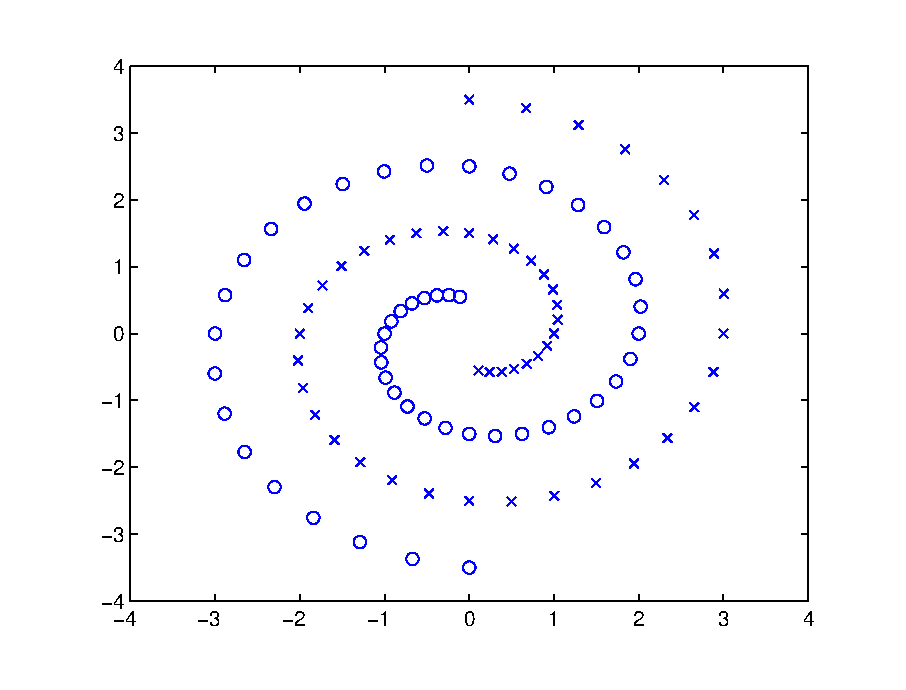
\epsfig{file=trainExamples.eps,width=0.9\columnwidth}
\caption{Training set examples plotting}
\end{figure}

The batch learning MLQPs model achieves 100 \% on both training set and testing set examples. The figure 2 shows the experiment result. Figure 3 illustrates the tends that cost function changed with iterations.

\begin{figure}
\centering
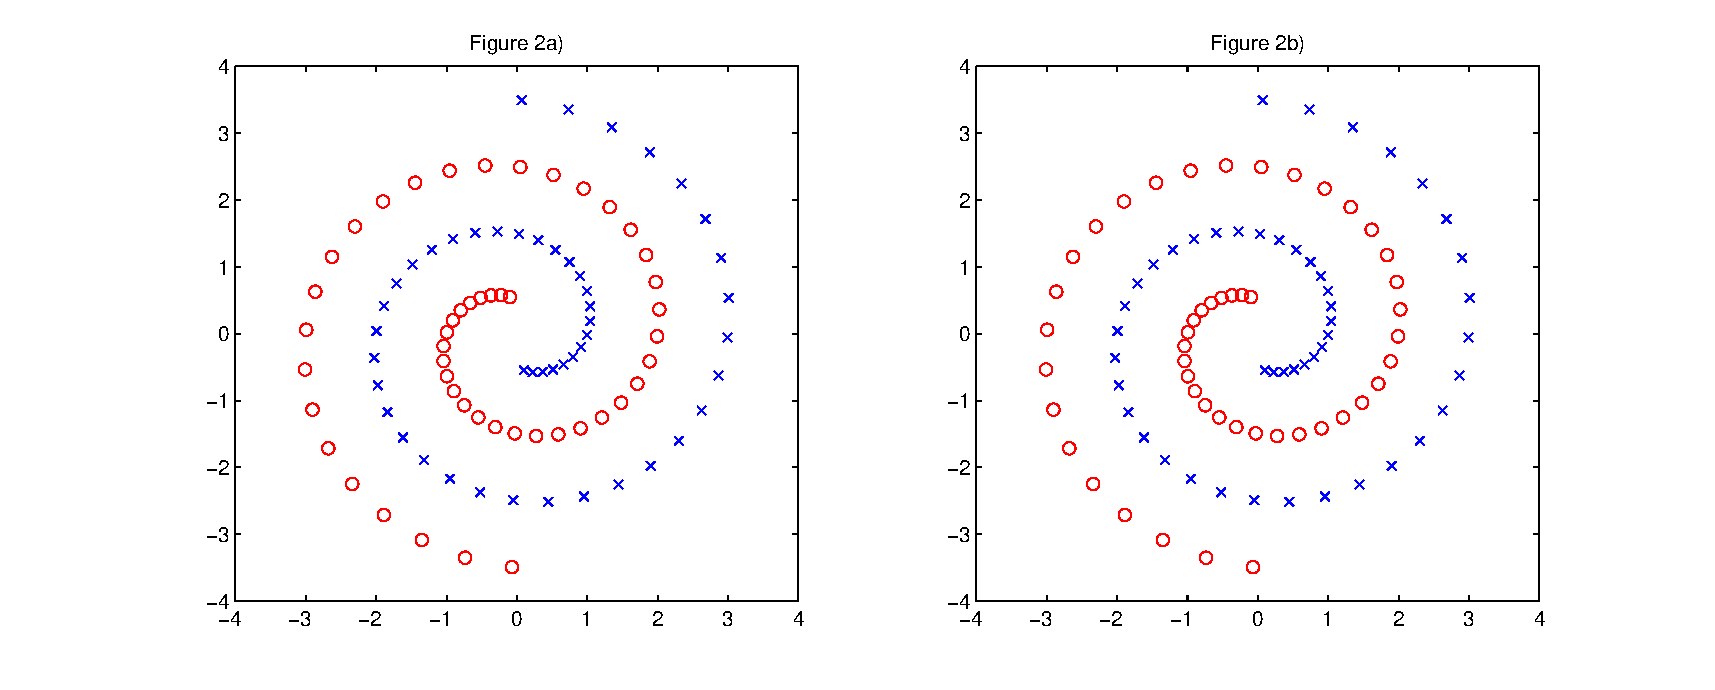
\epsfig{file=batchCompare.eps,width=\columnwidth}
\caption{Batch learning result on test set. Figure 2a) plot the test set examples; Figure 2b) plot the prediction result on the test set examples using batch learning MLQPs model}
\end{figure}

The precision of the result on test set examples using batch learning MLQPs model is 100 \%. We can see that Figure 2a) and Figure 2b) exactly match well on each other.

Figure 3 separately illustrates two different classification regions of MLQPs model for this training data set in red color and blue color.
\begin{figure}
\centering

\epsfig{file = decision.eps,width=0.9\columnwidth}
\caption{Decision Region, the red region and blue region represents for two different classes region in the problem. }
\end{figure}

We also do the experiment to compare the two algorithms (batch algorithm and online algorithm) for running time. Using the simple gradient descent optimization algorithm, the batch learning algorithm costs 19.227 seconds, while the online learning algorithm costs about 5.522 seconds. Both of the batch learning algorithm and the online learning algorithm have 100 \% precision. However, batch algorithm speeds up to 2.695 seconds after adopting the \textbf{advanced optimization} algorithm L-BFGS.


\section{Conclusion}
I implement a three-layer neural network with back propagation algorithm using both batch and online technique.
Now, I am familiar with the detailed structure of MLQPs models. That's what I have learned from this assignment. I'm very interested in neural network now. I plan to take my effort in deep learning technique in my further study. Thanks for Prof. Lu and our TA.
   

\end{document}

